% 平移示意：△ABC 与 平移后的 △A'B'C'，对应点连线 AA',BB',CC' 平行且相等
\documentclass[tikz,border=4pt]{standalone}
\usepackage{ctex}
\usepackage{amsmath}
\usetikzlibrary{calc, arrows.meta, decorations.markings}
\begin{document}
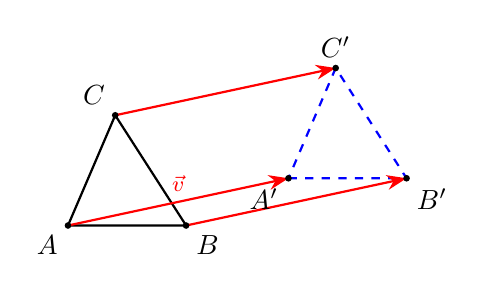
\begin{tikzpicture}[scale=1.0, thick]
  \coordinate (A) at (0,0);
  \coordinate (B) at (1.5,0);
  \coordinate (C) at (0.6,1.4);
  % 平移向量 v=(2.8,0.6)
  \coordinate (Ap) at (2.8,0.6);
  \coordinate (Bp) at (4.3,0.6);
  \coordinate (Cp) at (3.4,2.0);

  \draw (A) -- (B) -- (C) -- cycle;
  \draw[blue, dashed] (Ap) -- (Bp) -- (Cp) -- cycle;

  % 对应点连线
  \draw[red, -{Stealth[length=2.5mm]}] (A) -- (Ap);
  \draw[red, -{Stealth[length=2.5mm]}] (B) -- (Bp);
  \draw[red, -{Stealth[length=2.5mm]}] (C) -- (Cp);

  \fill (A) circle (1.2pt); \fill (B) circle (1.2pt); \fill (C) circle (1.2pt);
  \fill (Ap) circle (1.2pt); \fill (Bp) circle (1.2pt); \fill (Cp) circle (1.2pt);

  \node[below left] at (A)  {$A$};
  \node[below right] at (B) {$B$};
  \node[above left]  at (C) {$C$};
  \node[below left]  at (Ap) {$A'$};
  \node[below right] at (Bp) {$B'$};
  \node[above]       at (Cp) {$C'$};
  \node[red, above] at ($(A)!0.5!(Ap)$) {\footnotesize $\vec{v}$};
\end{tikzpicture}
\end{document}
